\documentclass{article}

\usepackage[margin=0.8in]{geometry}
\usepackage{subfig}
\usepackage{amsmath}
\usepackage{amsfonts}
\usepackage{amssymb}
\usepackage{amsthm}
\usepackage{graphicx}
\usepackage[hidelinks]{hyperref}
\usepackage{showlabels}
\usepackage{lineno}
% \linenumbers
\usepackage{natbib}

\newtheorem{lemma}{Lemma}
\newtheorem{prop}{Proposition}
\newtheorem{thm}{Theorem}
\newtheorem{prob}{Problem}
\newtheorem{defn}{Definition}
\newtheorem{obs}{Observation}
\newtheorem{alg}{Algorithm}

\newcommand{\median}{\operatorname{median}}

% http://bytesizebio.net/2013/03/11/adding-supplementary-tables-and-figures-in-latex/
\newcommand{\beginsupplement}{%
        \setcounter{table}{0}
        \renewcommand{\thetable}{S\arabic{table}}%
        \setcounter{figure}{0}
        \renewcommand{\thefigure}{S\arabic{figure}}%
     }

\hyphenation{Ge-nome Ge-nomes hyper-mut-ation through-put}

\title{Fall Internship Report: A literature review on quantitative assays immunology}
\author{Jared Galloway}

\begin{document}
\maketitle

\begin{abstract}
Protection from rapidly evolving and spreading viruses is key to human health and survival.
The molecular nature of infection and immune system defences provides us with a complex and noisy set of of problems to solve
if we are to combat infectious disease and understand the nature of their evolution.
Most notably, we need to understand the binding affinity of a virus to bind to a host cell via proteins on the expressed on the surface of the cell's outer membrane.
These proteins allow the virus to enter a host cell, then proceed to hijack the cell's own machinery to replicate and propagate an infection.
In the context of SARS-CoV-2, understanding the immune response with respect to those binding proteins is critical
for prevention and prediction of disease severity.
Additionally, understanding the evolution of these binding sites allows us to interpret the cross-species transmission
and duration of immunity post-infection, or the potential mutational routes of binding escape.
Neither of these are trivial problems to solve. 
Fortunately, recent advances in next generation sequencing (NGS), oligonucleotide synthesis (ONS), and PCR-induced <?>
have driven the development of quantitative assays and given us the ability to explore and quantify fitness of particular sequences in the context of protein interaction.
These methods have laid the foundation for exploration and development of advanced vaccines providing protection against deadly pathogens
from causing serious illness and even death.
In this literature review, we explore the advanced quantitative assays, Phage Immunoprecipitation Sequencing
and Deep Mutational Scanning, which allow us to measure and explore these complex and noisy problems.
Concretely, we will observe the results and methods from \citet{Shrock2020} and \citet{Starr2020}, two papers that focus on the binding properties of the novel betacoronavirus, SARS-CoV-2.
% Further we explore the modeling and analysis techniques necessary to parse and query the resulting data from these protocols.
\end{abstract}


\section*{Introduction}
% Hooray for Joe~\cite{Felsenstein1981-zs}.
Modern mammalian immune systems are constituted by the aggregate of proteins and cells which
defend against unwanted invaders (pathogens).
These defences keep the pathogens from harming the delicate and complex biological systems which keep us alive and healthy.
However, deadly pathogenic outbreaks which rapidly spread among humans and other species can often harm or kill a large percentage of populations \citep{Wu2020}.
In the case of viruses, replication as a function of fitness drives pathogens to evolve much in the same way we do --
often meaning the most potent and infectious pathogens prevail as a product of their genome evolution \citep{Twiddy2003, Felsenstein1981-zs}.
Fighting fire with fire, the adaptive immune system works through similar processes of mutation and selection, inside our own body,
to evolve along-side these pathogens and confer specialized immunity - in many cases lasting throughout the lifetime of an individual.
Incredibly, the combinatorial effects of specialized (VDJ) recombination results in enough diversity to select upon that evolution of specialized cells
takes place in mere days (often a week or so) when encountering a new pathogen \citep{Jung2004}.

~

As fast as this process works in contrast to all other forms of evolution (often on more ecological timescales), 
the symptoms of an infection can still make an individual very ill, or even be fatal .
Viruses are very good at hijacking our cells own machinery to replicate itself in order to propagate the infection.
The degree to which these pathogens can harm host cells is determined by the amount of time it takes your adaptive immune system to elicit the right responses and create
antibodies which can identify and induce destruction of pathogens and infected cells.
Once an individual has encountered a pathogen and created the necessary cells needed to fend off the virus and infected cells,
the defences that were used are stored in a sort of ``immuno-memory" -- using another type specialized cell.
Upon contact with a pathogen the individual has encountered in the past, then,
the immune system has the infrastructure in place to elicit a fast and effective response, known as a immunity.
One of the most impactful developments in human health has been our ability to provoke immune responses to common
viruses without actually infecting us with a deadly disease causing pathogen.
These biologically prepared agents are known as vaccines.

~

Commonly, a vaccine for some particular virus essentially models the virus - without any of the harmful properties.
This can be thought of as giving your immune system a molecular picture of the virus so that it is prepared when the real thing is encountered
Anything that elicits an immune response is known as an antigen, and the antigen for a particular pathogen is known as the epitope.
Knowing the epitope for any virus is key in modeling it for vaccines.
Inferring a particular antigen is no trivial process, the number of possible peptides chains forming a protein
which constitute the epitope for any particular virus are nearly infinitesimal.
To date there is no direct way to determine which proteins are expressed on a virus, and which constitute an antigen.
To complicate further, little is known about how sequence variation affects protein function.
As viruses evolve, we would like to know how possible mutations impact our immuno-defences.
In the case of the novel coronavirus, SARS-CoV-2, high mutation rates have already been found in the region which binds to our cells.
In order to predict or understand how long immunity will last in the face of evolution, we must explore all variants of the epitope
and their respective binding affinity relative to the wild type sequence.

~

Fortunately, recent advances in next generation sequencing (NGS), oligonucleotide synthesis (ONS), and PCR-induced 

Here, we dig into the benefits and limitations of two such quantitative assays, Phage Immunoprecipitation Sequencing (PhIP-Seq), 
and Deep Mutational Scanning (DMS) along with the analysis techniques we use to query the resulting data from these protocols.



\cite{Starr2020}


\section*{Quantitative assays}

\subsection*{Phage-Immuno Precipitation Sequencing}

%\begin{figure}
%\centering
%\begin{tabular}{cc}
%  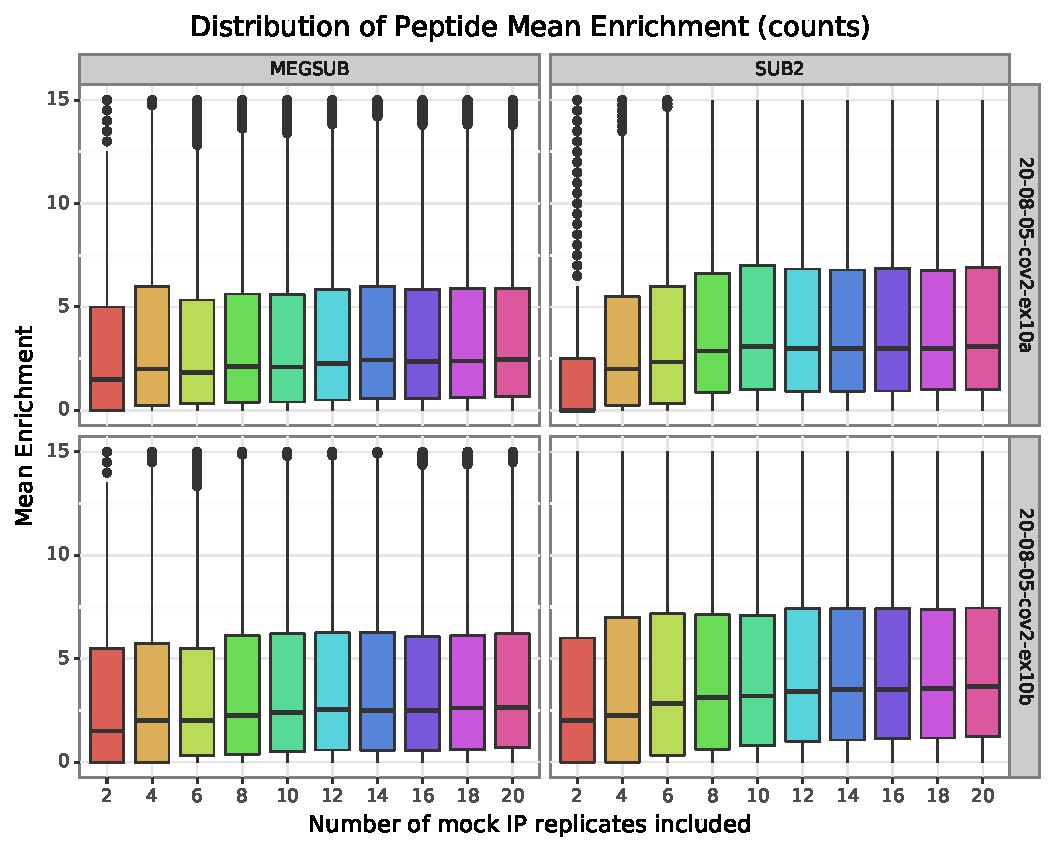
\includegraphics[width=85mm]{figures/42_mockip_abundance_variance/counts/mean_limit_y.pdf} &   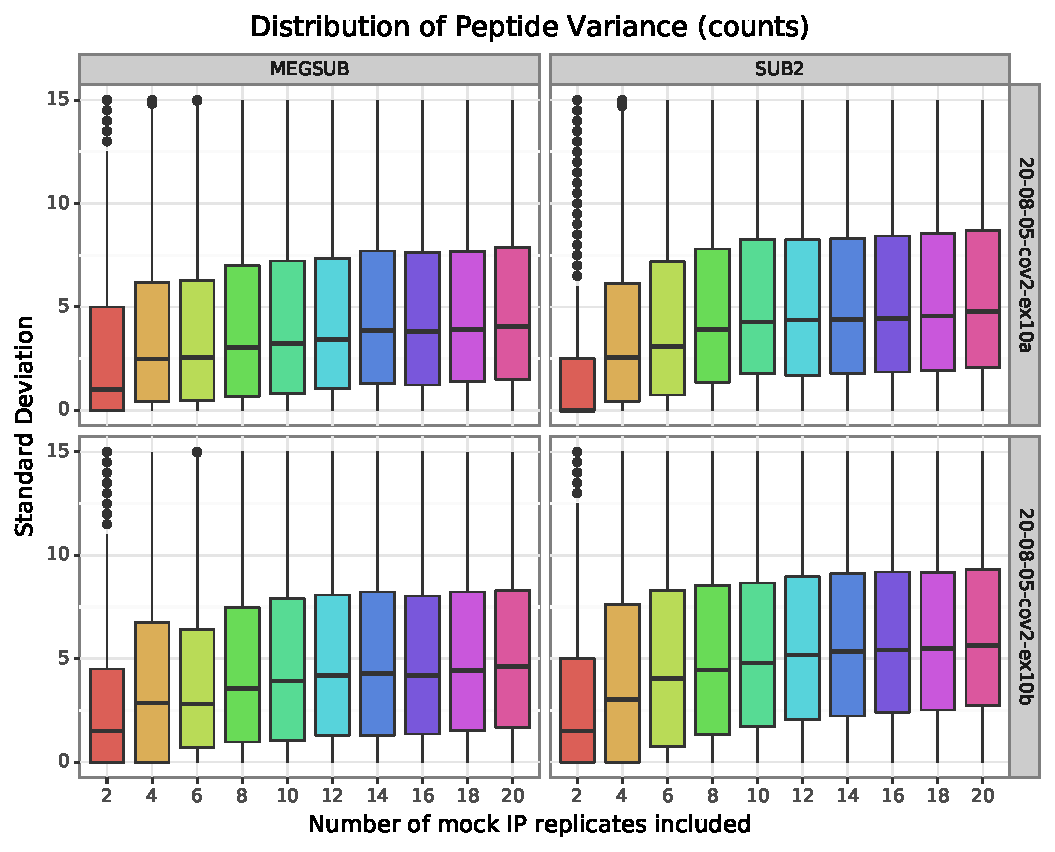
\includegraphics[width=85mm]{figures/42_mockip_abundance_variance/counts/std_limit_y.pdf} \\
%(a) first & (b) second \\[6pt]
% \includegraphics[width=85mm]{figures/42_mockip_abundance_variance/counts/mean.pdf} &   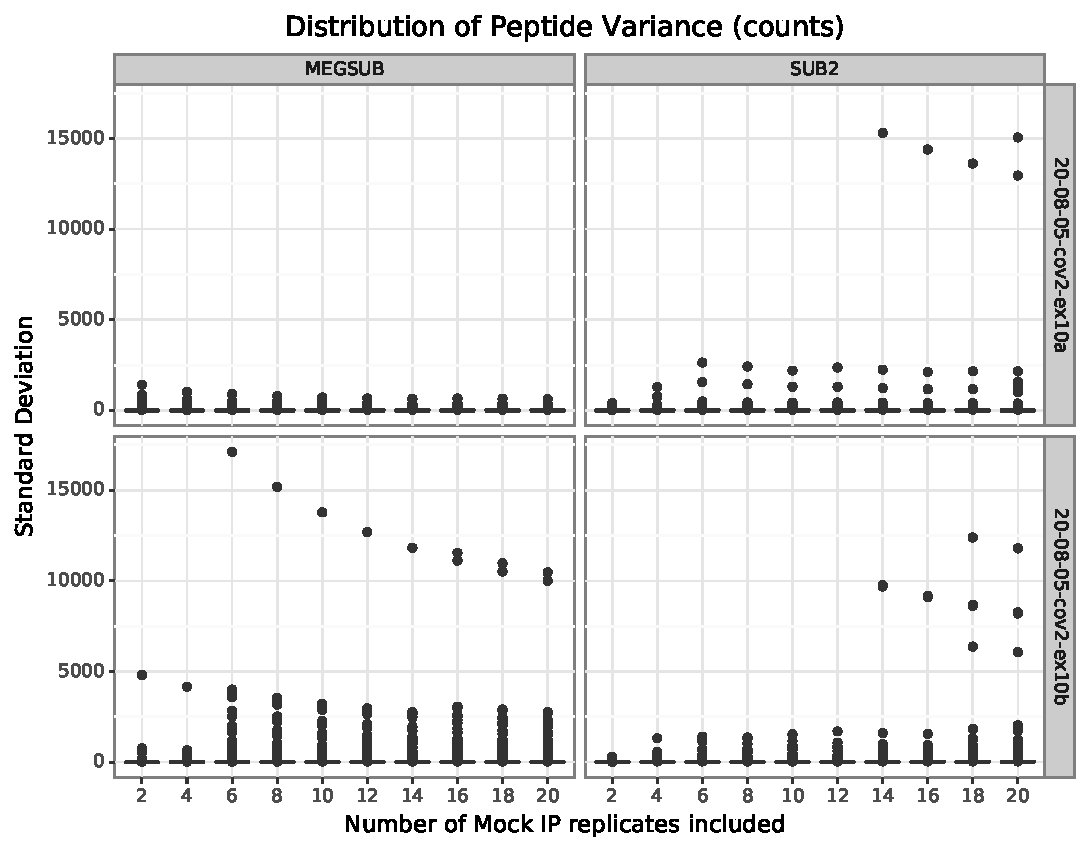
\includegraphics[width=85mm]{figures/42_mockip_abundance_variance/counts/std.pdf} \\
%(c) third & (d) fourth \\[6pt]
%\multicolumn{2}{c}{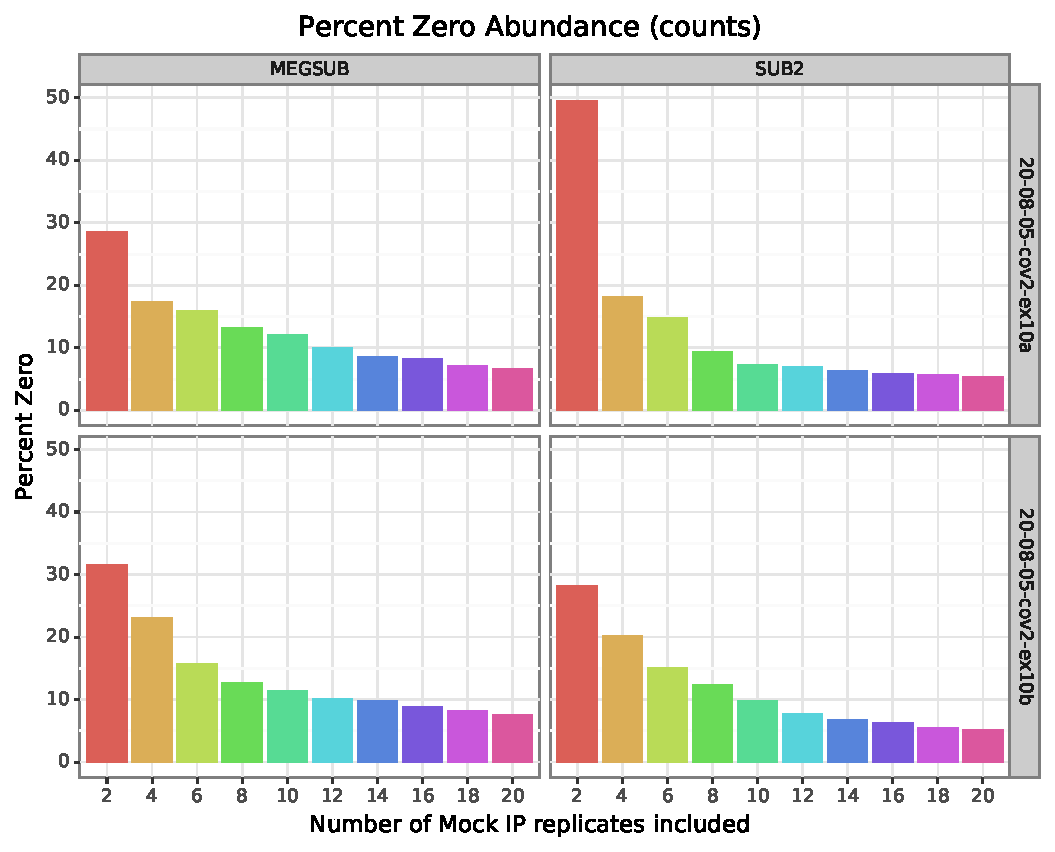
\includegraphics[width=105mm]{figures/42_mockip_abundance_variance/counts/per-zero.pdf} }\\
%\multicolumn{2}{c}{(e) fifth}
%\end{tabular}
%\caption{caption}
%\end{figure}
%
%\begin{figure}
%\centering
%\begin{tabular}{cc}
%  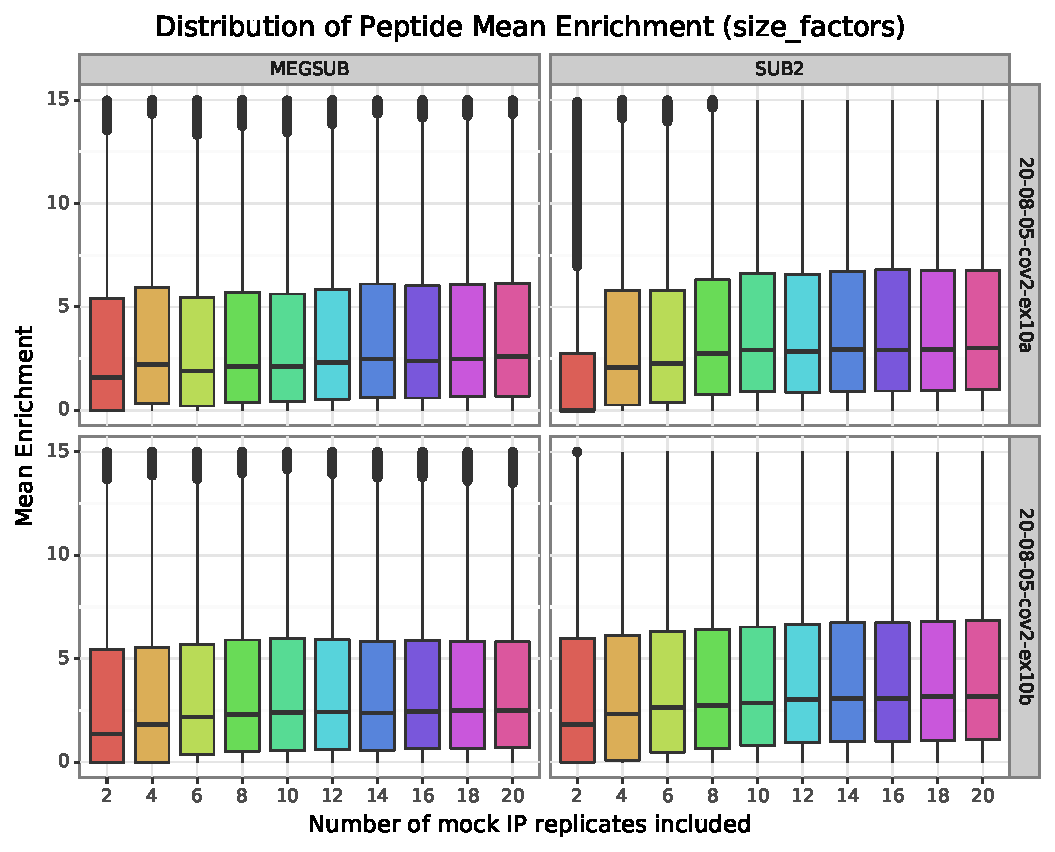
\includegraphics[width=85mm]{figures/42_mockip_abundance_variance/size_factors/mean_limit_y.pdf} &   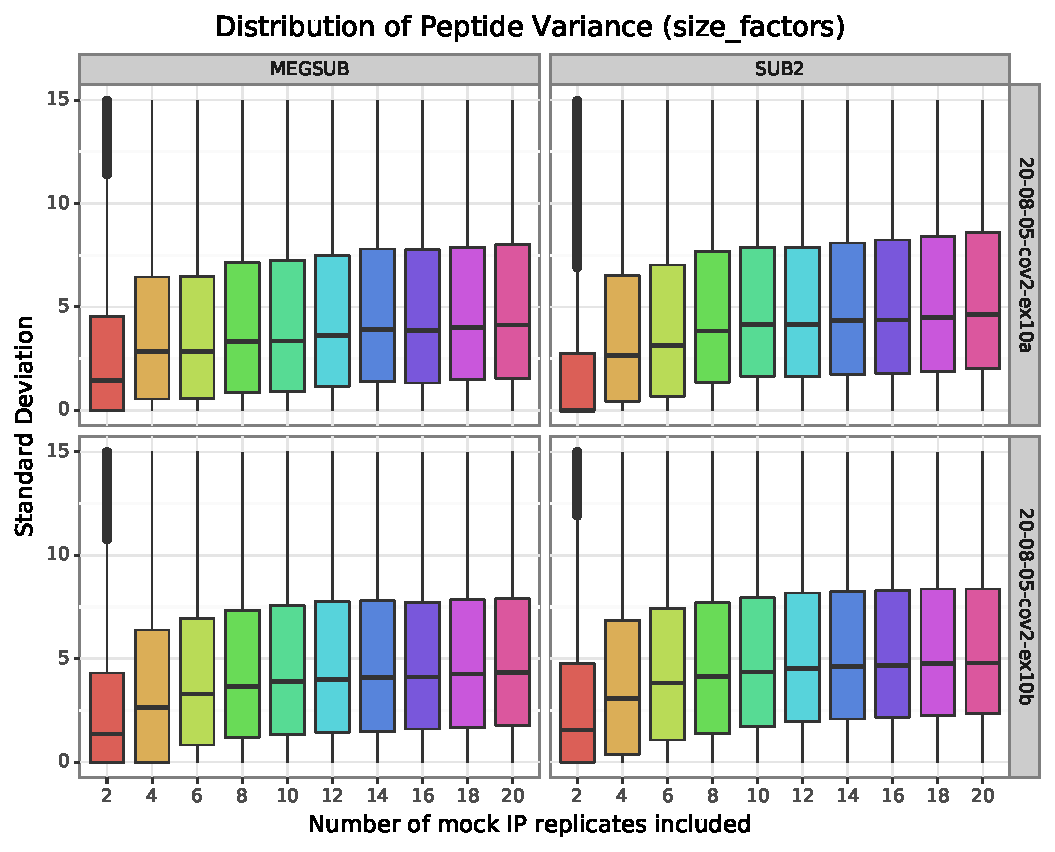
\includegraphics[width=85mm]{figures/42_mockip_abundance_variance/size_factors/std_limit_y.pdf} \\
%(a) first & (b) second \\[6pt]
% \includegraphics[width=85mm]{figures/42_mockip_abundance_variance/size_factors/mean.pdf} &   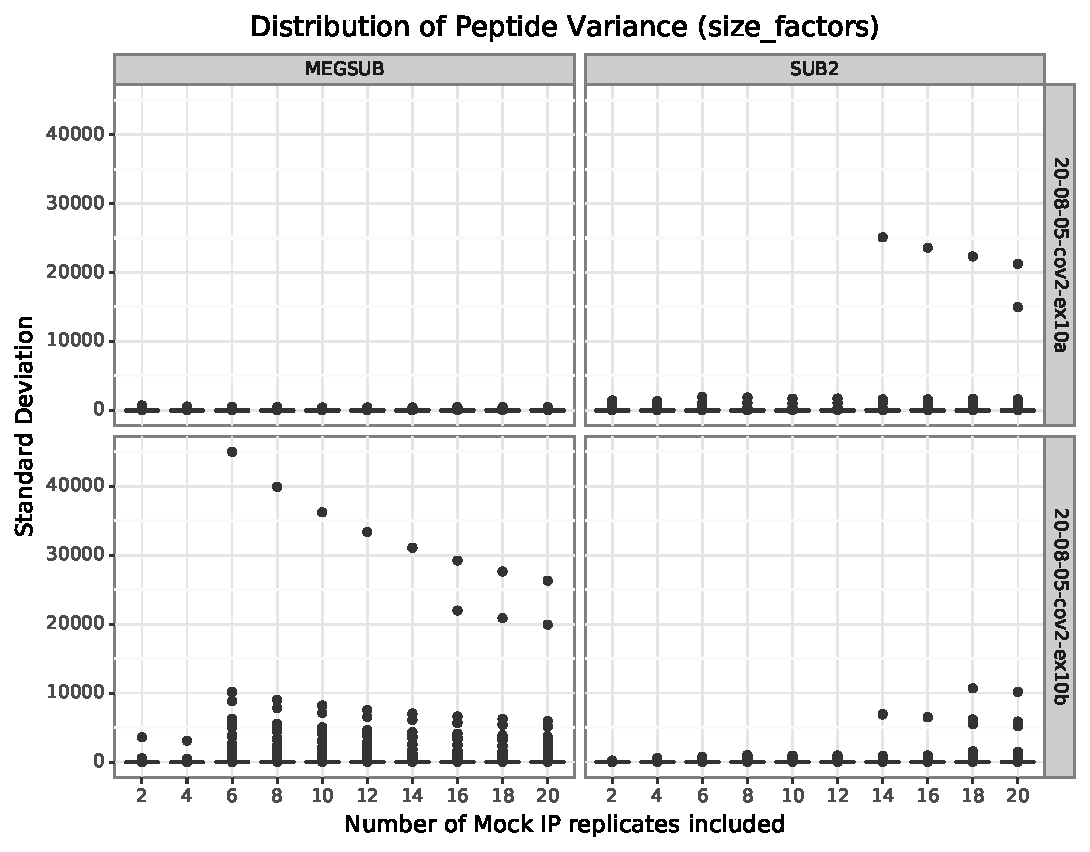
\includegraphics[width=85mm]{figures/42_mockip_abundance_variance/size_factors/std.pdf} \\
%(c) third & (d) fourth \\[6pt]
%\multicolumn{2}{c}{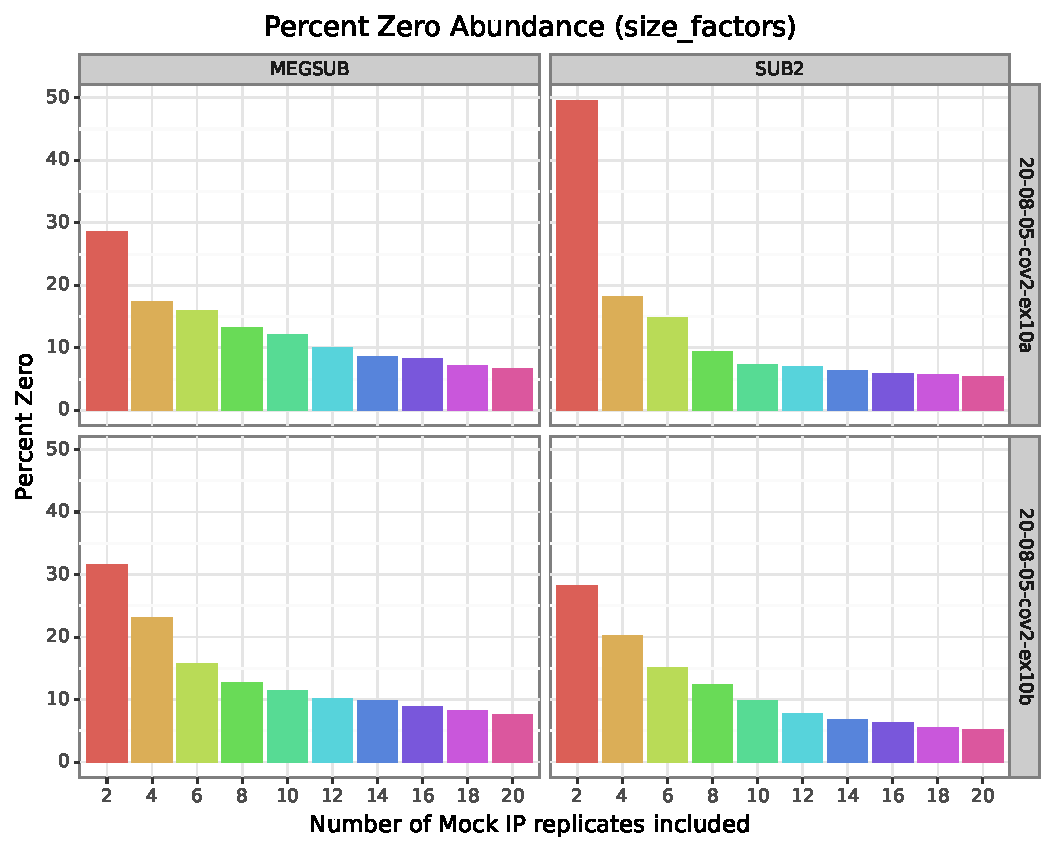
\includegraphics[width=105mm]{figures/42_mockip_abundance_variance/size_factors/per-zero.pdf} }\\
%\multicolumn{2}{c}{(e) fifth}
%\end{tabular}
%\caption{caption}
%\end{figure}

\subsection*{Deep Mutational Scanning}

\subsection*{Analysis and modeling}

\section*{Future Perspectives and Conclusions}




% \begin{figure}[h]
% \centering
% \includegraphics[width=0.35\textwidth]{figures/subsplit.pdf}
% \caption{\
% A subsplit structure.
% }%
% \label{fig:subsplit}
% \end{figure}


% \bibliographystyle{plain}
% \bibliography{main}

\bibliographystyle{plainnat}
\bibliography{main}

% \clearpage
% \section*{Supplementary Materials}
% \beginsupplement
% Supplementary text and figures here.


\end{document}
